\begin{definition}[\textbf{Ángulo:}]
Un ángulo es la unión de dos rayos no colineales que tienen el mismo origen.

\begin{figure}[!h]
    \centering
    \begin{tikzpicture}
    % Define los puntos
    \tkzDefPoint(0,0){A}
    \tkzDefPoint(3,0){B}
    \tkzDefPoint(1,2){C}
    
    % Dibuja los rayos AB y AC
    \tkzDrawSegment[-Latex](A,B)
    \tkzDrawSegment[-Latex](A,C)

    \tkzDefMidPoint(A,B) \tkzGetPoint{AMP}
    \tkzDefMidPoint(A,C) \tkzGetPoint{AMC}

    % Marca el vértice A
    \tkzLabelPoint[below](A){$A$}
    \tkzLabelPoint[below](AMP){$B$}
    \tkzLabelPoint[above left](AMC){$C$}

    \tkzDrawPoints(A,AMP,AMC)
    
    % Dibuja el ángulo BAC
    \tkzMarkAngle[arc=l, size=0.5cm](B,A,C)
\end{tikzpicture}
    \label{fig:angle}
    \caption{$\angle{BAC}$}
\end{figure}

\end{definition}

\begin{definition}[\textbf{Interior de un ángulo:}]
Dado un ángulo $\angle{AVC}$, el \textit{interior} de $\angle{AVC}$ es la intersección del semiplano determinado por $\ray{VC}$ que contiene a $A$ y el semiplano determinado por $\ray{VA}$ que contiene a $C$.

\end{definition}

\begin{definition}[\textbf{Exterior de un ángulo:}]
El exterior de $\angle{AVC}$ es el conjunto de todos los puntos que no están en el ángulo $\angle{AVC}$ ni en su interior.
\end{definition}
    
\begin{definition}[\textbf{Punto interior de un ángulo:}]
Sea el $\angle{AVC}$ en el plano $\pi$. El punto $D$ pertenece al interior de $\angle{AVC}$ si:

\begin{itemize}
    \item $A$ y $D$ están del mismo lado de la recta $\eline{VC}$.
    \item $C$ y $D$ están del mismo lado de la recta $\eline{VA}$.
\end{itemize}

\begin{figure}[h!]
    \centering
    \begin{subfigure}[b]{.5\textwidth}
        \centering
        \begin{tikzpicture}
    % Define los puntos
    \tkzDefPoint(0,0){A}
    \tkzDefPoint(3,0){B}
    \tkzDefPoint(1,2){C}
    \tkzDefPoint(1.5,0.8){D}
    
    % Dibuja los rayos AB y AC
    \tkzDrawSegment[-Latex](A,B)
    \tkzDrawSegment[-Latex](A,C)

    \tkzDefMidPoint(A,B) \tkzGetPoint{AMP}
    \tkzDefMidPoint(A,C) \tkzGetPoint{AMC}

    % Marca el vértice A
    \tkzLabelPoint[below](A){$V$}
    \tkzLabelPoint[below](AMP){$C$}
    \tkzLabelPoint[above left](AMC){$A$}
    \tkzLabelPoint[right](D){$D$}
    
    \tkzDrawPoints(AMP,AMC,D)
    
    % Dibuja el ángulo BAC
    \tkzMarkAngle[arc=l, size=0.5cm](B,A,C)
\end{tikzpicture}
        \caption{Ángulo interior}
        \label{fig:ang-interior}
    \end{subfigure}%
    \begin{subfigure}[b]{.5\textwidth}
        \centering
        \begin{tikzpicture}
    % Define los puntos
    \tkzDefPoint(0,0){A}
    \tkzDefPoint(3,0){B}
    \tkzDefPoint(1,2){C}
    \tkzDefPoint(0,2){D}
    
    % Dibuja los rayos AB y AC
    \tkzDrawSegment[-Latex](A,B)
    \tkzDrawSegment[-Latex](A,C)

    \tkzDefMidPoint(A,B) \tkzGetPoint{AMP}
    \tkzDefMidPoint(A,C) \tkzGetPoint{AMC}

    % Marca el vértice A
    \tkzLabelPoint[below](A){$V$}
    \tkzLabelPoint[below](AMP){$C$}
    \tkzLabelPoint[above left](AMC){$A$}
    \tkzLabelPoint[left](D){$D$}
    
    \tkzDrawPoints(AMP,AMC,D)
    
    % Dibuja el ángulo BAC
    \tkzMarkAngle[arc=l, size=0.5cm](B,A,C)
\end{tikzpicture}
        \caption{Ángulo exterior}
        \label{fig:ang-exterior}
    \end{subfigure}
    \centering
    \label{fig:ang-int-ext}
\end{figure}    

\end{definition}

\begin{postulate}[\textbf{Medida de ángulos:}]
    A cada ángulo le corresponde un único número real entre $0^{\circ}$ y $180^{\circ}$.

\begin{figure}[!h]
    \centering
    \begin{tikzpicture}
    % Define los puntos
    \tkzDefPoint(0,0){A}
    \tkzDefPoint(3,0){B}
    \tkzDefPoint(1,2){C}
    
    % Dibuja los rayos AB y AC
    \tkzDrawSegment[-Latex](A,B)
    \tkzDrawSegment[-Latex](A,C)

    \tkzDefMidPoint(A,B) \tkzGetPoint{AMP}
    \tkzDefMidPoint(A,C) \tkzGetPoint{AMC}

    % Marca el vértice A
    \tkzLabelPoint[below](A){$A$}
    \tkzLabelPoint[below](AMP){$B$}
    \tkzLabelPoint[above left](AMC){$C$}

    \tkzDrawPoints(AMP,AMC)
    
    % Dibuja el ángulo BAC
    \tkzMarkAngle[arc=l, size=0.5cm](B,A,C)
    \tkzLabelAngle[pos = 0.9](B,A,C){$\degs{r}$}
\end{tikzpicture}
    \label{fig:ang-medida}
    \caption{Medida de un ángulo}
    \caption{$m\angle{BAC}=\degs{r}$}
\end{figure}

\end{postulate}

\clearpage

\begin{definition}[\textbf{Ángulos congruentes:}]
    Dos o más ángulos son \textit{congruentes} si tienen la misma medida.
\end{definition}


\begin{postulate}[\textbf{Construcción de ángulos:}]
    Sea $H$ un plano y $\ray{AB}$ un rayo de la arista del plano $H_1$. Para cada número real $\degrees{r}$ entre $\degrees{0}$ y $\degrees{180}$ hay exactamente un rayo $\ray{AP}$, con $P \in H_1$, tal que $m\angle{PAB} = \degrees{r}$.

    \begin{figure}[!h]
        \centering
        \begin{tikzpicture}
    % Define los puntos
    \tkzDefPoint(0,0){A}
    \tkzDefPoint(3,0){B}
    \tkzDefPoint(1,2){C}

    \tkzDefPoint(-2,0){D}
    \tkzDefPoint(1.5,1.5){H1}
    
    % Dibuja los rayos AB y AC
    \tkzDrawSegment[-Latex](A,B)
    \tkzDrawSegment[-Latex](A,C)

    \tkzDefMidPoint(A,B) \tkzGetPoint{AMP}
    \tkzDefMidPoint(A,C) \tkzGetPoint{AMC}

    % Marca el vértice A
    \tkzLabelPoint[below](A){$A$}
    \tkzLabelPoint[below](AMP){$B$}
    \tkzLabelPoint[above left](AMC){$P$}

    \tkzLabelPoint(H1){$\scriptsize{H_1}$}

    \tkzDrawPoints(A,AMP,AMC)
    
    % Dibuja el ángulo BAC
    \tkzMarkAngle[arc=l, size=0.5cm](B,A,C)
    \tkzLabelAngle[pos = 0.9](B,A,C){$\degs{r}$}

    \tkzDrawSegment[dashed,-Latex](A,D)
\end{tikzpicture}
        \label{fig:ang-construct}
    \end{figure}
    
\end{postulate}

\begin{postulate}[\textbf{Adición de ángulos:}]
    Si el punto $C$ está en el interior de $\angle{ABD}$, entonces $m\angle{ABD} = m\angle{ABC} + m\angle{CBD}$. De igual forma $m\angle{ABC} = m\angle{ABD} - m\angle{CBD}$.


    \begin{figure}[!h]
        \centering
        \begin{tikzpicture}

    % Define los puntos
    \tkzDefPoint(0,0){A}
    \tkzDefPoint(3,0){B}
    \tkzDefPoint(0,3){C}
    \tkzDefPoint(3,3){D}
    
    % Dibuja las líneas AB, BC y BD
    \tkzDrawSegment[Latex-](A,B)
    \tkzDrawSegment[-Latex](B,C)
    \tkzDrawSegment[-Latex](B,D)

    \tkzDefMidPoint(A,B) \tkzGetPoint{MAB}
    \tkzDefMidPoint(B,C) \tkzGetPoint{MBC}
    \tkzDefMidPoint(B,D) \tkzGetPoint{MBD}

    % Marca los puntos
    \tkzLabelPoint[below left](MAB){$A$}
    \tkzLabelPoint[below right](B){$B$}
    \tkzLabelPoint[above right](MBC){$C$}
    \tkzLabelPoint[above right](MBD){$D$}

    \tkzDrawPoints(MAB,MBC,MBD)

\end{tikzpicture}
        \label{fig:ang-suma}
        \caption{$m\angle{ABD} = m\angle{ABC} + m\angle{CBD}$}
    \end{figure}
    
\end{postulate}

\begin{postulate}
    Todos los ángulos rectos son congruentes.
    
    \begin{figure}[!h]
        \centering
        \begin{tikzpicture}[scale=1] 
    % TRIANGULO 1
    \tkzDefPoints{% x    y   nombre
                    0  /0   /B,
                    0  /2   /A,
                    2  /0   /C,
                    0  /3   /D,
                    3  /0   /E}
    
    \tkzDrawPoints(A,B,C)
    \tkzLabelPoint[left](A){$A$}
    \tkzLabelPoint[below left](B){$B$}
    \tkzLabelPoint[below](C){$C$}
    
    \tkzDrawSegment[-Triangle](B,D)
    \tkzDrawSegment[-Triangle](B,E)
    \tkzMarkRightAngle[size=0.5](A,B,C)
    
    
    % TRIANGULO 2
    \tkzDefPoints{% x    y   nombre
                    5  /0   /F,
                    5  /1   /G,
                    9  /0   /H,
                    5  /2   /I,
                    10 /0   /J}
    
    
    \tkzDrawPoints(F,G,H)
    \tkzLabelPoint[below left](F){$E$}
    \tkzLabelPoint[left](G){$D$}
    \tkzLabelPoint[below](H){$F$}
    
    \tkzDrawSegment[-Triangle](F,I)
    \tkzDrawSegment[-Triangle](F,J)
    \tkzMarkRightAngle[size=0.5](G,F,H)
\end{tikzpicture}

        \caption{Ángulos rectos congruentes}
        \label{fig:ang-rect-cong}
    \end{figure}
    
\end{postulate}

\begin{definition}[\textbf{Ángulo agudo:}]
    Un ángulo agudo es aquel cuya medida es menor que $\degrees{90}$.
\end{definition}

\begin{definition}[\textbf{Ángulo obtuso:}]
    Un ángulo obtuso es aquel cuya medida es mayor que $\degrees{90}$.
\end{definition}

\begin{definition}[\textbf{Ángulo recto:}]
    Un ángulo recto es aquel que mide $\degrees{90}$.
\end{definition}

\clearpage

\begin{theorem}[\textbf{Teorema de la construcción de ángulos:}]
    Sea $\angle{ABC}$ y $\alpha$ un semiplano cuyo borde contiene a $\ray{DE}$, entonces hay exactamente un rayo $\ray{DF}$, con $F$ en $\alpha$, tal que $\angle{ABC} \cong \angle{FDE}$.

    \begin{figure}[h!]
    
        \centering
    
        \begin{subfigure}[b]{.3\textwidth}
            \centering
            \begin{tikzpicture}
    % Define los puntos
    \tkzDefPoint(0,0){A}
    \tkzDefPoint(3,0){B}
    \tkzDefPoint(1,2){C}
    
    % Dibuja los rayos AB y AC
    \tkzDrawSegment[-Latex](A,B)
    \tkzDrawSegment[-Latex](A,C)

    \tkzDefMidPoint(A,B) \tkzGetPoint{AMP}
    \tkzDefMidPoint(A,C) \tkzGetPoint{AMC}

    % Marca el vértice A
    \tkzLabelPoint[below](A){$B$}
    \tkzLabelPoint[below](AMP){$C$}
    \tkzLabelPoint[above left](AMC){$A$}

    \tkzDrawPoints(AMP,AMC)
    
    % Dibuja el ángulo BAC
    \tkzMarkAngle[arc=l, size=0.5cm](B,A,C)
    \tkzLabelAngle[pos = 0.9](B,A,C){$\degs{x}$}

    
\end{tikzpicture}
            \label{fig:plot108}
        \end{subfigure}%
        \begin{subfigure}[b]{.3\textwidth}
            \centering
            \begin{tikzpicture}
    % Define los puntos
    \tkzDefPoint(0,0){A}
    \tkzDefPoint(3,0){B}
    \tkzDefPoint(1,2){C}
    \tkzDefPoint(2.5,1){D}
    
    % Dibuja los rayos AB y AC
    \tkzDrawSegment[-Latex](A,B)
    \tkzDrawSegment[-Latex,dashed](A,C)

    \tkzDefMidPoint(A,B) \tkzGetPoint{AMP}
    \tkzDefMidPoint(A,C) \tkzGetPoint{AMC}

    % Marca el vértice A
    \tkzLabelPoint[below](A){$D$}
    \tkzLabelPoint[below](AMP){$E$}
    \tkzLabelPoint[above left](AMC){$F$}

    \tkzLabelPoint[above left](D){$\alpha$}

    \tkzDrawPoints(AMP,AMC)
    
    % Dibuja el ángulo BAC
    \tkzMarkAngle[arc=l, size=0.5cm](B,A,C)
    \tkzLabelAngle[pos = 0.9](B,A,C){$\degs{x}$}

    
\end{tikzpicture}
            \label{fig:plot109}
        \end{subfigure}

        \caption{Construcción de ángulos}
        \label{fig:ang-const-teorema}
        
    \end{figure}        
    
\end{theorem}

\begin{definition}[\textbf{Ángulos complementarios:}]
    Dos ángulos son complementarios si la suma de sus medidas es igual a $\degrees{90}$.
\end{definition}

\begin{definition}[\textbf{Ángulos suplementarios:}]
    Dos ángulos son complementarios si la suma de sus medidas es igual a $\degrees{180}$.
\end{definition}

\begin{theorem}[\textbf{Ángulos complementarios:}]
    Si dos ángulos son complementarios, entonces ambos son agudos.
\end{theorem}

\begin{theorem}[\textbf{Complementos congruentes:}]
    Si dos ángulos son complemento de ángulos congruentes, entonces son congruentes entre sí.
\end{theorem}

\begin{theorem}[\textbf{Suplementos congruentes:}]
    Si dos ángulos son suplemento de ángulos congruentes, entonces son congruentes entre sí.
\end{theorem}

\begin{definition}[\textbf{Ángulos adyacentes:}]
    Dos ángulos $\angle{ABC}$ y $\angle{CBD}$ se llaman adyacentes si tienen un lado en común y los lados no comunes pertenecen a los semiplanos opuestos determinados por la recta que contiene el lado común.
\end{definition}

\begin{definition}[\textbf{Rayos opuestos:}]
    Sean $A,B$ y $C$ puntos de una recta $l$. Si $A$ está entre $B$ y $C$, entonces $\ray{AB}$ y $\ray{AC}$ se llaman rayos opuestos.

    \begin{figure}[!h]
        \centering
        \begin{tikzpicture}
    
    % Define los puntos
    \tkzDefPoint(0,0){C}
    \tkzDefPoint(3,0){A}
    \tkzDefPoint(6,0){B}
    
    % Dibuja línea l
    \tkzDrawLine[add=0.5 and 0.5,Latex-Latex](C,B) 
    \tkzLabelLine[above,pos=1.2](C,B){$l$} 

    % Etiqueta los puntos
    \tkzLabelPoint[below](C){$C$}
    \tkzLabelPoint[below](A){$A$}
    \tkzLabelPoint[below](B){$B$}

    \tkzDrawPoints(C,A,B)

    % Dibuja y etiqueta los segmentos CA y AB
    \tkzDrawSegment(C,A)
    \tkzLabelSegment[above](C,A){$\ray{AC}$}
    \tkzDrawSegment(A,B)
    \tkzLabelSegment[above](A,B){$\ray{AB}$}
\end{tikzpicture}
        \caption{Rayos opuestos}
        \label{fig:rayos-opuesto}
    \end{figure}
    
\end{definition}

\clearpage

\begin{definition}[\textbf{Par lineal:}]
    Dos ángulos forman un par lineal si los ángulos tienen un lado en común y los otros dos lados son rayos opuestos.

\end{definition}

\begin{postulate}[\textbf{Ángulos suplementarios del par lineal}]
    Si dos ángulos forman un par lineal, entonces los ángulos son suplementarios.
\end{postulate}

\begin{theorem}[\textbf{Par lineal de ángulos rectos:}]
    Si en un par lineal un ángulo es recto, entonces el otro también es recto.
\end{theorem}

\begin{figure}[!h]
    \centering
    \begin{tikzpicture}
    % Definir los puntos del ángulo
    \tkzDefPoint(0,0){B}
    \tkzDefPoint(-2,0){A}
    \tkzDefPoint(2,0){D}
    \tkzDefPoint(1,2){C}

    % Dibujar los ángulos
    \tkzDrawSegment[add=0.2 and 0.2,Latex-Latex](A,D)
    \tkzDrawSegment[add=0 and 0.2,-Latex](B,C)

    % Marcar los puntos
    \tkzDrawPoints(A,B,C,D)
    \tkzLabelPoint[below left](A){$A$}
    \tkzLabelPoint[below](B){$B$}
    \tkzLabelPoint[left](C){$C$}
    \tkzLabelPoint[below right](D){$D$}

    % Marcar los ángulos
    \tkzMarkAngle[size=0.8](D,B,C)
    \tkzLabelAngle[pos=0.6](D,B,C){$\alpha$}

    \tkzMarkAngle[size=0.8](C,B,A)
    \tkzLabelAngle[pos=0.4](C,B,A){$\beta$}

\end{tikzpicture}


    \caption{Par lineal: $\alpha + \beta = \degs{180}$}
    \label{fig:par-lineal}
\end{figure}    

\begin{definition}[\textbf{Ángulos opuestos por el vértice:}]
    Dos ángulos son opuestos por el vértice si sus lados forman dos pares de rayos opuestos.
\end{definition}

\begin{theorem}[\textbf{Ángulos opuestos por el vértice:}]
    Ángulos opuestos por el vértice son congruentes.

    \begin{figure}[!h]
        \centering
        \begin{tikzpicture}[scale=0.8]
    % Definir los puntos
    \tkzDefPoint(0,0){A}
    \tkzDefPoint(-2,2){B}
    \tkzDefPoint(2,2){C}
    \tkzDefPoint(-2,-2){D}
    \tkzDefPoint(2,-2){E}

    % Dibujar las lineas y puntos
    \tkzDrawSegment[add=0 and 0.2,-Latex](A,B)
    \tkzDrawSegment[add=0 and 0.2,-Latex](A,C)
    \tkzDrawSegment[add=0 and 0.2,-Latex](A,D)
    \tkzDrawSegment[add=0 and 0.2,-Latex](A,E)
    
    \tkzDrawPoints(A,B,C,D,E)

    % Marcar los puntos
    \tkzLabelPoint[below left](B){$B$}
    \tkzLabelPoint[below right](C){$C$}
    \tkzLabelPoint[above right](E){$E$}
    \tkzLabelPoint[above left](D){$D$}
    \tkzLabelPoint[below](A){$A$}

    % Marcar los ángulos
    \tkzMarkAngle[arc=l,size=0.8,mark=|,color=red](B,A,D)
    \tkzMarkAngle[arc=l,size=0.8,mark=|,color=red](E,A,C)

    \tkzMarkAngle[arc=l,size=0.8,mark=||,color=blue](C,A,B)
    \tkzMarkAngle[arc=l,size=0.8,mark=||,color=blue](D,A,E)

\end{tikzpicture}
        \caption{Ángulos opuestos por el vértice}
        \label{fig:ang-opuestos}
    \end{figure}
    
\end{theorem}

\begin{theorem}[\textbf{Intersección de ángulos rectos:}]
    Si dos rectas que se intersecan determinan un ángulo recto, entonces los otros tres ángulos definidos por esas rectas también son rectos.
\end{theorem}


